


\tikzset{every picture/.style={line width=0.75pt}} %set default line width to 0.75pt        

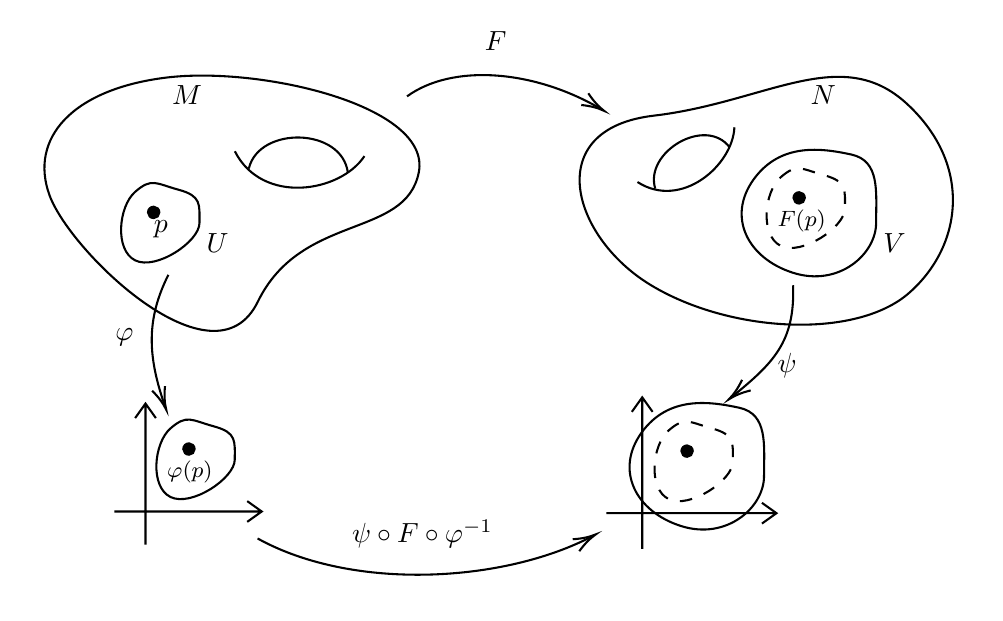
\begin{tikzpicture}[x=0.75pt,y=0.75pt,yscale=-1,xscale=1]
%uncomment if require: \path (0,308); %set diagram left start at 0, and has height of 308

%Shape: Polygon Curved [id:ds6525401307539842] 
\draw   (172.32,39.91) .. controls (217.93,34.42) and (300.03,53.64) .. (293.65,85.68) .. controls (287.26,117.72) and (237.09,104.91) .. (216.11,147.93) .. controls (195.13,190.95) and (125.8,124.13) .. (115.76,96.67) .. controls (105.73,69.21) and (126.71,45.41) .. (172.32,39.91) -- cycle ;
%Curve Lines [id:da13910221661848143] 
\draw    (205.05,75.45) .. controls (218.2,101.5) and (255.9,95.36) .. (267.47,77.78) ;
%Curve Lines [id:da7264884996321357] 
\draw    (211.78,83.77) .. controls (216.62,63.2) and (256.67,63.81) .. (259.5,85.79) ;
%Shape: Ellipse [id:dp09144271455218123] 
\draw  [fill={rgb, 255:red, 0; green, 0; blue, 0 }  ,fill opacity=1 ] (163.2,104.91) .. controls (163.2,103.39) and (164.42,102.16) .. (165.94,102.16) .. controls (167.45,102.16) and (168.67,103.39) .. (168.67,104.91) .. controls (168.67,106.42) and (167.45,107.65) .. (165.94,107.65) .. controls (164.42,107.65) and (163.2,106.42) .. (163.2,104.91) -- cycle ;

%Curve Lines [id:da40516895320740165] 
\draw    (399.04,90.27) .. controls (420.05,103.85) and (444.95,82.27) .. (445.73,63.89) ;
%Shape: Polygon Curved [id:ds6664506251612305] 
\draw   (406.83,58.3) .. controls (461.29,51.9) and (497.08,23.13) .. (528.98,52.7) .. controls (560.89,82.27) and (555.44,121.43) .. (529.76,143.81) .. controls (504.09,166.19) and (443.39,162.99) .. (405.27,139.81) .. controls (367.14,116.64) and (352.36,64.69) .. (406.83,58.3) -- cycle ;
%Curve Lines [id:da7681269690042121] 
\draw    (407.6,93.46) .. controls (402.16,75.88) and (431.72,58.3) .. (443.39,73.48) ;
%Shape: Polygon Curved [id:ds13343779797680644] 
\draw   (157,95) .. controls (165,88) and (167,91) .. (178,94) .. controls (189,97) and (188,101) .. (188,110) .. controls (188,119) and (167,133) .. (157,128) .. controls (147,123) and (149,102) .. (157,95) -- cycle ;
%Shape: Polygon Curved [id:ds6611856882220029] 
\draw   (455,89) .. controls (468,71) and (488,74) .. (502,77) .. controls (516,80) and (514,95) .. (514,110) .. controls (514,125) and (496,141) .. (474,134) .. controls (452,127) and (442,107) .. (455,89) -- cycle ;
%Curve Lines [id:da20913952032416394] 
\draw    (288,49) .. controls (309.67,33.24) and (348.8,35.91) .. (381.51,55.11) ;
\draw [shift={(383,56)}, rotate = 211.22] [color={rgb, 255:red, 0; green, 0; blue, 0 }  ][line width=0.75]    (10.93,-3.29) .. controls (6.95,-1.4) and (3.31,-0.3) .. (0,0) .. controls (3.31,0.3) and (6.95,1.4) .. (10.93,3.29)   ;
%Shape: Ellipse [id:dp28625789196692764] 
\draw  [fill={rgb, 255:red, 0; green, 0; blue, 0 }  ,fill opacity=1 ] (180.2,218.91) .. controls (180.2,217.39) and (181.42,216.16) .. (182.94,216.16) .. controls (184.45,216.16) and (185.67,217.39) .. (185.67,218.91) .. controls (185.67,220.42) and (184.45,221.65) .. (182.94,221.65) .. controls (181.42,221.65) and (180.2,220.42) .. (180.2,218.91) -- cycle ;
%Shape: Polygon Curved [id:ds6638368612589451] 
\draw   (174,209) .. controls (182,202) and (184,205) .. (195,208) .. controls (206,211) and (205,215) .. (205,224) .. controls (205,233) and (184,247) .. (174,242) .. controls (164,237) and (166,216) .. (174,209) -- cycle ;
%Curve Lines [id:da41107146503736036] 
\draw    (173,135) .. controls (162.27,156.45) and (162.96,174.1) .. (171.34,198.14) ;
\draw [shift={(172,200)}, rotate = 250.2] [color={rgb, 255:red, 0; green, 0; blue, 0 }  ][line width=0.75]    (10.93,-3.29) .. controls (6.95,-1.4) and (3.31,-0.3) .. (0,0) .. controls (3.31,0.3) and (6.95,1.4) .. (10.93,3.29)   ;
%Shape: Ellipse [id:dp45763550840932554] 
\draw  [fill={rgb, 255:red, 0; green, 0; blue, 0 }  ,fill opacity=1 ] (474.2,97.91) .. controls (474.2,96.39) and (475.42,95.16) .. (476.94,95.16) .. controls (478.45,95.16) and (479.67,96.39) .. (479.67,97.91) .. controls (479.67,99.42) and (478.45,100.65) .. (476.94,100.65) .. controls (475.42,100.65) and (474.2,99.42) .. (474.2,97.91) -- cycle ;
%Shape: Polygon Curved [id:ds9301475980831604] 
\draw  [dash pattern={on 4.5pt off 4.5pt}] (468,88) .. controls (476,81) and (478,84) .. (489,87) .. controls (500,90) and (499,94) .. (499,103) .. controls (499,112) and (478,126) .. (468,121) .. controls (458,116) and (460,95) .. (468,88) -- cycle ;
%Curve Lines [id:da1605123699723061] 
\draw    (474,140) .. controls (474.98,167.44) and (464.44,177.59) .. (444.25,193.99) ;
\draw [shift={(443,195)}, rotate = 321.01] [color={rgb, 255:red, 0; green, 0; blue, 0 }  ][line width=0.75]    (10.93,-3.29) .. controls (6.95,-1.4) and (3.31,-0.3) .. (0,0) .. controls (3.31,0.3) and (6.95,1.4) .. (10.93,3.29)   ;
%Curve Lines [id:da5075807557158749] 
\draw    (216,262) .. controls (262.53,287.74) and (335.52,283.1) .. (377.73,260.68) ;
\draw [shift={(379,260)}, rotate = 151.29] [color={rgb, 255:red, 0; green, 0; blue, 0 }  ][line width=0.75]    (10.93,-3.29) .. controls (6.95,-1.4) and (3.31,-0.3) .. (0,0) .. controls (3.31,0.3) and (6.95,1.4) .. (10.93,3.29)   ;
%Shape: Axis 2D [id:dp1641739751745317] 
\draw  (147,249) -- (218,249)(162,197) -- (162,265) (211,244) -- (218,249) -- (211,254) (157,204) -- (162,197) -- (167,204)  ;
%Shape: Axis 2D [id:dp7431220916836756] 
\draw  (384,249.82) -- (466,249.82)(401.32,194) -- (401.32,267) (459,244.82) -- (466,249.82) -- (459,254.82) (396.32,201) -- (401.32,194) -- (406.32,201)  ;
%Shape: Polygon Curved [id:ds06622774826865241] 
\draw   (401,211) .. controls (414,193) and (434,196) .. (448,199) .. controls (462,202) and (460,217) .. (460,232) .. controls (460,247) and (442,263) .. (420,256) .. controls (398,249) and (388,229) .. (401,211) -- cycle ;
%Shape: Ellipse [id:dp6760122392287706] 
\draw  [fill={rgb, 255:red, 0; green, 0; blue, 0 }  ,fill opacity=1 ] (420.2,219.91) .. controls (420.2,218.39) and (421.42,217.16) .. (422.94,217.16) .. controls (424.45,217.16) and (425.67,218.39) .. (425.67,219.91) .. controls (425.67,221.42) and (424.45,222.65) .. (422.94,222.65) .. controls (421.42,222.65) and (420.2,221.42) .. (420.2,219.91) -- cycle ;
%Shape: Polygon Curved [id:ds3192888406480947] 
\draw  [dash pattern={on 4.5pt off 4.5pt}] (414,210) .. controls (422,203) and (424,206) .. (435,209) .. controls (446,212) and (445,216) .. (445,225) .. controls (445,234) and (424,248) .. (414,243) .. controls (404,238) and (406,217) .. (414,210) -- cycle ;

% Text Node
\draw (173.36,42.38) node [anchor=north west][inner sep=0.75pt]    {$M$};
% Text Node
\draw (190,113.4) node [anchor=north west][inner sep=0.75pt]    {$U$};
% Text Node
\draw (164.5,107.38) node [anchor=north west][inner sep=0.75pt]    {$p$};
% Text Node
\draw (324,16.4) node [anchor=north west][inner sep=0.75pt]    {$\mathnormal{F}$};
% Text Node
\draw (170.94,223.05) node [anchor=north west][inner sep=0.75pt]  [font=\footnotesize]  {$\varphi ( p)$};
% Text Node
\draw (146,159.4) node [anchor=north west][inner sep=0.75pt]    {$\varphi $};
% Text Node
\draw (481,42.4) node [anchor=north west][inner sep=0.75pt]    {$\mathnormal{N}$};
% Text Node
\draw (465,102.4) node [anchor=north west][inner sep=0.75pt]  [font=\footnotesize]  {$F( p)$};
% Text Node
\draw (516,113.4) node [anchor=north west][inner sep=0.75pt]    {$V$};
% Text Node
\draw (465,171.4) node [anchor=north west][inner sep=0.75pt]    {$\psi $};
% Text Node
\draw (260,251.4) node [anchor=north west][inner sep=0.75pt]    {$\psi \circ F\circ \varphi ^{-1}$};


\end{tikzpicture}
